%\RequirePackage[l2tabu, orthodox]{nag}  %Checks for older packages 

\documentclass[11pt,a4paper]{article}
% \documentclass[10pt]{extreport} $ allos to make the font smaller
\usepackage[utf8]{inputenc}

\usepackage{amsmath}
\usepackage{amsfonts}
\usepackage{indentfirst}
\usepackage{amssymb}
\usepackage[font={footnotesize}]{caption} %Makes the captions small


%% Figures packages
\usepackage[pdftex]{graphicx}
\usepackage{float}   %Es para colocar el objeto flotante exactamente donde se ponga el comando con H
\usepackage{caption}
\usepackage{subcaption}
\graphicspath{{../results/}}
\usepackage{sidecap}  %Para poner figuras a los lados


\usepackage{setspace} % Needed for Pyton syntax highlight
\usepackage{listings}    % Include the listings-package, nice verbatim for code
\usepackage{color}
\usepackage{courier}


\usepackage{cleveref} %puts figure and equation appropiately \cref{} 

\usepackage{natbib} %For bibliography
%\usepackage{cite}
\usepackage{framed} % To use boxes, or frames around text

\usepackage{parskip} %Para saltos entre parrafos
\setlength{\parindent}{0pt} 
\setlength{\parskip}{\baselineskip}
\usepackage[a4paper,margin=0.8in]{geometry}  %%Cambiar los margenes

\newcommand{\HRule}{\rule{\linewidth}{0.5mm}}

%\usepackage{hyperref} %This should be loade after most of the other packages 
% \hypersetup{colorlinks=true}  %Para que los hiperlinks cuando se hagan referencias aparezcan en colores.

\definecolor{dkgreen}{rgb}{0,0.6,0}

\title{Lab12: DD2380 }
\author{
Ramon Heberto Martinez Mayorquin  hramon@kth.se 
}



\begin{document}

\begin{titlepage}
\begin{center}
%\includegraphics[width=0.15\textwidth]{logo}\\[1cm]    

\textsc{\LARGE Kungliga Tekniska högskolan}\\[1.0cm]

\textsc{\Large Computational Python 2015}\\[2.0cm]



\begin{figure}[H]
	\centering
 
\includegraphics[width=0.35\textwidth]{sese.png}
\end{figure}
%\\[1cm]    
%

% Title
\HRule \\[0.4cm]
{ \huge  Parameter Exploration for in-house library.
}\\[0.4cm]
\HRule \\[1.5cm]

% Author and supervisor

Author: Ram\'on  Mart\'inez  \\ 
\large Course Responsible: Olav Vahtras  \\ [2.5cm]
%\normalsize Presenta \\
%\large Supervisors 2: Jan Antolik \\[2.5cm]

\textsc{\Large School of Computer Science and Communication \\
PDC Center for High Performance Computing}\\ [1.0cm] 
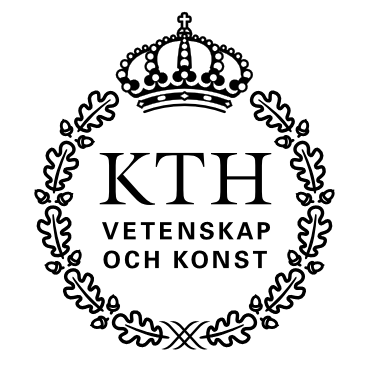
\includegraphics[width=0.15\textwidth]{KTH_black.png}\\[1.5cm] % Controls the distance till the new object 
% Bottom of the page
{\large 17th November of 2015}

\end{center}
\end{titlepage}



\begin{abstract}
This report is used to describe our work regarding tools for parameter
exploration in an in-house library. First we describe the data
processing pipeline that we use in this research. This describes the rather complicated process to make it more manageable and furthermore introduces the context. Once we do we can present the pairs of input and output that we want to store and describe the problem around this process. To conclude we provide more technical details on how the how process is carried out. 
\end{abstract}


\section{Problem.}\label{problem.}

\subsection{Spatio-temporal Structure}\label{spatio-temporal-structure}

We have a in-house library that functions mainly as a big pipeline for
data processing and exploration. The input of the data pipeline is composed of $N_{time\:series}$ time series each one with a sampling rate attached to it. To each of those time series we attach what we a \textbf{lag structure}. The lag structure is a vector that
represents \textbf{how we believe the past of the signal affects the
present}. In more detail, the vector contains a series of lags that we
use to calculate the auto-correlation between the time series and the
time series shifted by quantities given on this vector. For example if the vector of lags is
the following lags = (1, 2, 3, ... ) then we can obtain the usual
auto-correlation function because all this shifts are given by the unit. In general we use the same lag vector for every signal and we will denote the dimension of that vector here as
($N_{lags}$) for further explanations.

In our use case the signals come from different points in space, so they
encode the spatial information. By adding a law vector to each signal we
intend to include also spatial information between them. Our aim is to
quantify how the different points in space are related between
themselves in space and time. In order to do so we calculate a
cross-correlation matrix. For each possible lag and every possible
signal combination we calculate the cross-correlation between them. This
way we obtain a matrix with ($N_{time series} \times (N_{lags}$)
rows and the same amount of columns. We call this matrix the Spatio
Temporal Distance Matrix (\textbf{STDM}) and it provides a concrete
measure of the spatio-temporal relationships.

Finally we would like to interpret our spatio-temporal relationships as
a distance matrix. In the example above an given entry is going to be
big if the elements that represent the row and the column are highly
correlated. This is exactly the opposite of what we want. We want our
\textbf{elements to be far away if they are uncorrelated and to cluster
together if they are correlated}. So in order to interpret them as
distances we create another matrix where each entry is one minus the
absolute value of the old matrix. This way we can directly interpret
this matrix as a distance measure between the spatial and temporal parts
of the whole input space as we initially intended.

\subsubsection{Embedding}\label{embedding}

At this stage of our analysis we have a distance matrix that represents
how all the sensors and the shifted in time versions of those sensors
related. The next step in our pipeline is to apply the Multidimensional
Scaling Algorithm (\textbf{MDS}) in order to embed all the ($N_{time
series} \times (N_{lags})$ points in an euclidean space of dimension
\(N_{embed}\) that we chose.

\subsubsection{Spatial-Temporal
Clustering.}\label{spatial-temporal-clustering.}

Now with all our points into our euclidean space we can partition our
sensor space by a process of vector quantization. Here we have to
determine the number of partition or cluster with another parameter
decided by ourselves \(N_{spatial clusters}\). After this process is
done we have each of the sensors and their respective lags associated
with a particular clusters. In other words what we have created is a
division of the spatio-temporal information according to the data it
provides.

\subsubsection{Data clustering.}\label{data-clustering.}

The final point is to partition the data as well. For each of the
clusters above we select a number \(N_{data clusters}\) that quantifies
how many clusters the data in that space will have. So for a given group
of sensor we consider all the data on that particular group and apply a
cluster algorithm to it.

\subsection{Parameters.}\label{parameters.}

The first things that stands out with the description above is the sheer
complexity of the problem. There are many bifurcations in the pipeline
and in order to cope with this complexity we need to come up with a
systematic way of dealing with the parameters. In the following we
identify that parameter that we must setup before running the pipeline
and the data at the output that we we want to store and associate with
it.

\subparagraph{Input parameters.}\label{input-parameters.}

\begin{itemize}
\item
  Data (This is also the data that characterizes the signal)
\item
  \(N_{spatial clusters}\)
\item
  \(N_{embedding space}\)
\item
  \(N_{data clusters}\)
\item
  lag\_structure (t\_i, window\_size, filter)
\item
  time, dt
\item
  Git Version
\end{itemize}

\subparagraph{Output data to
visualize.}\label{output-data-to-visualize.}

\begin{itemize}
\item
  Matrix with the signals lagged
\item
  STDM
\item
  A map from each of the sensors to the cluster that it belongs.
\item
  The embedding of all the sensors in the euclidean space.
\item
  The center of the clusters in the data space.
\item
  A map that assigns to each spatial clustering a set of data clusters.
\end{itemize}

\subsubsection{The main problem.}\label{the-main-problem.}

The main problem is here is to attach to our pipeline a mechanism to
understand the role of the parameter in the data processing mechanisms.
In order to do so we need a systematized way of consistently storing the
data with the relevant parameters attach to it. Our first attempt at it
is just to produce a plot for each of the relevant graphs above. In the
following section I describe how this can be done using
\texttt{matpltlotlib}, version control and the tools that we learn to
use in the course.

\subsection{Python used and python
learned.}\label{python-used-and-python-learned.}

\subsubsection{Git branches}\label{git-branches}

The first thing to describe regarding the tools used in the course is
version control. I have been using version control before but I was
doing it in a monolotical and mono-branch way. This created problems
because if a new feature was created that deviated far enough from the
original (and working) project it was really hard to backtrack
appropriately. By creating a different branch in order to work with
experimental setups the whole process gets isolated and if things go out
of control too much reverting back to business as usual is as easy as
changing branch and deleting the experiment. So in brief I learnt how to
use multiple branches at git in order to deal experimental feature
development.

\subsubsection{Matplotlib}\label{matplotlib}

In order to take full advantage of the configuration of matplotlib it is
necessary to use it in its class oriented mode. For the visualization
tools for example I had the following problem. When I first started
using the pipeline I created a function to display everyone of the
quantities above and only one of them. However, when I wanted to do the
parameter exploration I realized that it would be very handy to combine
these plots into multigrid substructure (by this I mean the grid that
you get when you do something like subplot). So I had a dilemma. Doing
that in the most straightforward way would imply building new functions
(one for each pair of relevant plots that I wanted to combine) in order
to display these two figures at the same time. This however went
directly against the principle of do not repeat yourself. Furthermore
what if down the line I wanted to combine three instead of two figures
in one plot. if that was the case I will have to build yet another
function for each of the triplets and you can see from the combinatorial
explosion that this is not going to end up well.

The way around this problem was to study in detail the matplotlib object
model in detail. We realize then that the in matplotlib we can decouple
the canvas from the contents of the draw that we put in the canvas, in
matplotlib parlance we can just construct an axis like plot or an image
and then position them wherever we want into he canvas later with an
appropriate function. In short instead of coding again a function for
each of the plots we only make our normal functions to accept an axis as
an argument and if not figure is available we attach all the usual
content to the axis and return it. After returning we can position the
axis freely on the canvas with Gridspec for example or any other
convenience function that is fit for the job.

\subsubsection{Decoupling of data products and data
visualization}\label{decoupling-of-data-products-and-data-visualization}

Yet another problem with our pipeline is the amount of memory and
computing time that it takes in order to go through even a simple
example. This means that doing the usual process of generating all the
data and gathering the complete output for all the possible parameters
was out of question. The solution to that is \textbf{to decouple the
data generation process from the data visualization}. In this case we
first create the plots for a given combination of parameters and store
them. As the name of the file we use a string that involves a
combination of all the parameter used to create the signal. We save all
of those images in a folder with a timestamp as title in order to make
the run unique and for logging process.

Now that we have all the set of images with a string characterizing
their parameters as a tittle we can access them systematically. The
classical way of doing this will be construct a GUI that just controls
the parameters and extracts the image with the unique string.
Fortunately Python provides an even faster way of doing the same tasks.
We can use the Ipython.widgets module in order to create sliders for
those parameters or a combination of them. In short using the ipython
notebook we have created and interactive environment that retrieves the
image that we need and displays it automatically allowing a smooth
exploration of parameters without the hassle of building a GUI to
achieve this.

\subsection{Final Discussion.}\label{final-discussion.}

We have describe here the process of building a parameter exploration
library. The tools that have helped us accomplishing this goal are the
class oriented capabilities of the matplotlib library and the
interactivity added to ipython notebook with the widgets package. With
those two and decoupling the generation from the visualization of our
data we can construct complex routines, let them running and study the
results later in an interactive way.

A problem with this approach is that the images that we store take quite
a bit space and are not reproducible. That is, the step from data to
image is irreversible. A further step ahead will be to store the data
instead of the images as the end results of our pipeline. A project that
looks very interesting to us in that regard is the \texttt{h5py}
project. The project provides an API to write and read to the hdf5
format in a clean and pythonic way. Using this tool we could store all
the homogeneous data produced with our simulations and store the
parameters as attributes in the data model of hdf5. We hope to build
that for our next step.


\bibliographystyle{plainnat}
\bibliography{references}
\end{document}
